%  LaTeX support: latex@mdpi.com 
%  In case you need support, please attach all files that are necessary for compiling as well as the log file, and specify the details of your LaTeX setup (which operating system and LaTeX version / tools you are using).

% You need to save the "mdpi.cls" and "mdpi.bst" files into the same folder as this template file.

%=================================================================
\documentclass[entropy,article,submit,moreauthors,pdftex,10pt,a4paper]{mdpi} 

%
%--------------------
% Class Options:
%--------------------
% journal
%----------
% Choose between the following MDPI journals:
% actuators, admsci, aerospace, agriculture, agronomy, algorithms, animals, antibiotics, antibodies, antioxidants, applsci, arts, atmosphere, atoms, axioms, batteries, behavsci, beverages, bioengineering, biology, biomedicines, biomimetics, biomolecules, biosensors, brainsci, buildings, carbon, cancers, catalysts, cells, challenges, chemosensors, children, chromatography, climate, coatings, computation, computers, condensedmatter, cosmetics, cryptography, crystals, data, dentistry, designs, diagnostics, diseases, diversity, econometrics, economies, education, electronics, energies, entropy, environments, epigenomes, fermentation, fibers, fishes, fluids, foods, forests, futureinternet, galaxies, games, gels, genealogy, genes, geosciences, geriatrics, healthcare, horticulturae, humanities, hydrology, informatics, information, infrastructures, inorganics, insects, instruments, ijerph, ijfs, ijms, ijgi, ijtpp, inventions, jcdd, jcm, jdb, jfb, jfmk, jimaging, jof, jintelligence, jlpea, jmse, jpm, jrfm, jsan, land, languages, laws, life, literature, lubricants, machines, magnetochemistry, marinedrugs, materials, mathematics, mca, mti, medsci, medicines, membranes, metabolites, metals, microarrays, micromachines, microorganisms, minerals, molbank, molecules, mps, nanomaterials, ncrna, neonatalscreening, nutrients, particles, pathogens, pharmaceuticals, pharmaceutics, pharmacy, philosophies, photonics, plants, polymers, processes, proteomes, publications, recycling, religions, remotesensing, resources, risks, robotics, safety, sensors, separations, sexes, sinusitis, socsci, societies, soils, sports, standards, sustainability, symmetry, systems, technologies, toxics, toxins, tropicalmed, universe, urbansci, vaccines, vetsci, viruses, water
%---------
% article
%---------
% The default type of manuscript is article, but can be replaced by: 
% addendum, article, book, bookreview, briefreport, casereport, changes, comment, commentary, communication, conceptpaper, correction, conferenceproceedings, conferencereport, expressionofconcern, meetingreport, creative, datadescriptor, discussion, editorial, essay, erratum, hypothesis, interestingimage, letter, newbookreceived, opinion, obituary, projectreport, reply, retraction, review, preprints, shortnote, supfile, technicalnote
% supfile = supplementary materials
%----------
% submit
%----------
% The class option "submit" will be changed to "accept" by the Editorial Office when the paper is accepted. This will only make changes to the frontpage (e.g. the logo of the journal will get visible), the headings, and the copyright information. Also, line numbering will be removed. Journal info and pagination for accepted papers will also be assigned by the Editorial Office.
%------------------
% moreauthors
%------------------
% If there is only one author the class option oneauthor should be used. Otherwise use the class option moreauthors.
%---------
% pdftex
%---------
% The option pdftex is for use with pdfLaTeX. If eps figure are used, remove the option pdftex and use LaTeX and dvi2pdf.

%=================================================================
\firstpage{1} 
\makeatletter 
\setcounter{page}{\@firstpage} 
\makeatother 
\articlenumber{x}
\doinum{10.3390/------}
\pubvolume{xx}
\pubyear{2016}
\copyrightyear{2016}
\externaleditor{Academic Editor: name}
\history{Received: date; Accepted: date; Published: date}

%------------------------------------------------------------------
% The following line should be uncommented if the LaTeX file is uploaded to arXiv.org
%\pdfoutput=1

%=================================================================
% Add packages and commands here. The following packages are loaded in our class file: fontenc, calc, indentfirst, fancyhdr, graphicx, lastpage, ifthen, lineno, float, amsmath, setspace, enumitem, mathpazo, booktabs, titlesec, etoolbox, amsthm, hyphenat, natbib, hyperref, footmisc, geometry, caption, url, mdframed

%=================================================================
%% Please use the following mathematics environments: Theorem, Lemma, Corollary, Proposition, Characterization, Property, Problem, Example, ExamplesandDefinitions, Remark, Definition
%% For proofs, please use the proof environment (the amsthm package is loaded by the MDPI class).

%=================================================================
% Full title of the paper (Capitalized)
\Title{EEG characterization and classification based on the histograms of visual gradients of plots}

% Authors, for the paper (add full first names)
\Author{Rodrigo Ramele $^{1,\dagger,\ddagger}$, Ana Julia Villar $^{1,\ddagger}$ and Juan Miguel Santos  $^{1,\ddagger}$*}
% Authors, for metadata in PDF
\AuthorNames{Rodrigo Ramele, Ana Julia Villar and Juan Miguel Santos}

% Affiliations / Addresses (Add [1] after \address if there is only one affiliation.)
\address[1]{%
$^{1}$ \quad Computer Engineering Department, Instituto Tecnológico de Buenos Aires (ITBA); info@itba.edu.ar}

% Contact information of the corresponding author
\corres{Correspondence: rramele@itba.edu.ar; Tel.: +54-9-11-4193-9382}

% Current address and/or shared authorship
\firstnote{Current address: C1437FBH Lavarden 315, Ciudad Autónoma de Buenos Aires, Argentina} 
\secondnote{These authors contributed equally to this work.}

% Simple summary
%\simplesumm{}

% Abstract (Do not use inserted blank lines, i.e. \\) 
\abstract{A single paragraph of about 200 words maximum. For research articles, abstracts should give a pertinent overview of the work. We strongly encourage authors to use the following style of structured abstracts, but without headings: 1) Background: Place the question addressed in a broad context and highlight the purpose of the study; 2) Methods: Describe briefly the main methods or treatments applied; 3) Results: Summarize the article's main findings; and 4) Conclusion: Indicate the main conclusions or interpretations. The abstract should be an objective representation of the article, it must not contain results which are not presented and substantiated in the main text and should not exaggerate the main conclusions.This is great.  We had tremendous results.  Our results are so great that nobody will believe that we actually managed to have them !}

% Keywords
\keyword{EEG; BCI; P300; ALS; classification; hog; sift}

% The fields PACS, MSC, and JEL may be left empty or commented out if not applicable
%\PACS{J0101}
%\MSC{}
%\JEL{}
%\AMS{}

% If this is an expanded version of a conference paper, please cite it here: enter the full citation of your conference paper, and add $^\S$ in the end of the title of this article.
%\conference{}

%%%%%%%%%%%%%%%%%%%%%%%%%%%%%%%%%%%%%%%%%%
% Only for the journal Data:

%\dataset{DOI number or link to the deposited data set in cases where the data set is published or set to be published separately. If the data set is submitted and will be published as a supplement to this paper in the journal Data, this field will be filled by the editors of the journal. In this case, please make sure to submit the data set as a supplement when entering your manuscript into our manuscript editorial system.}

%\datasetlicense{license under which the data set is made available (CC0, CC-BY, CC-BY-SA, CC-BY-NC, etc.)}

%%%%%%%%%%%%%%%%%%%%%%%%%%%%%%%%%%%%%%%%%%
% For Conference Proceedings Papers: add the conference title here
%\conferencetitle{}

%\setcounter{secnumdepth}{4}
%%%%%%%%%%%%%%%%%%%%%%%%%%%%%%%%%%%%%%%%%%
\begin{document}

%%%%%%%%%%%%%%%%%%%%%%%%%%%%%%%%%%%%%%%%%%
%% Only for the journal Gels: Please place the Experimental Section after the Conclusions

%%%%%%%%%%%%%%%%%%%%%%%%%%%%%%%%%%%%%%%%%%
\setcounter{section}{-1} %% Remove this when starting to work on the template.

\section{Introduction}

\begin{enumerate}[leftmargin=*,labelsep=3mm]
\item	Why
\item	Purpose and significance
\item	Current state of the research field and key publications cited
\item   Controversial hypothesis
\item   Main aim and principal conclusions.
\end{enumerate}

\begin{enumerate}[leftmargin=*,labelsep=3mm]
\item El paper tiene un foco general en EEG y rapidamente se centra en BCI como una prueba del método.
\item La relevancia de estudiar métodos de análisis de EEG para pacientes con ALS.
\item Ofrece una Receta de cómo implementar un esquema simple de detección de P300 y ofrece una comparativa contra el paper de las italianas.
\item La transversalidad del método de poder detectar eventos rítmicos asi como transientes como p300.
\item La posibilidad de utilizarlo para reconocer, fuertemente un patron particular y con la flexibilidad de detectar variantes basado en las poblaciones de descriptores (esta es mi hipótesis de porque funciona, porque yo vi que el método se hace pelota con pequeñas variantes de la señal).
\item La importancia del averaging de EEG y sus desbalanceos, puntualizando que en el paper original
\item Que la caída en la clasificación no cae significativamente aún bajando la cantidad de repeticiones requeridas para el averaging.
\item ¿ Por qué da mejor en PO8 que en Cz y Pz que son los canales P300 ?  (como future work).
\end{enumerate}



Although recently impressive advances in neuroimagining techniques has pushed EEG, Electroencephalography technology a little bit out of the way in clinical context, where it has always being used since its discovery by Berger.

Their versatility, ease of use, temporal resolution, ease and development of fabrication, and the explosion as a consumer devices, is pushing EEG devices to become the de-facto non invasive method to access and harness brain information.

Key contribution to this development has been the field of Brain Computer Interfaces, which is the development of a new channel of communication particularly aimed to person with some degree of neuro degenerative disease.

One very remarkable aspect of this communication channel is the ability to volitionally transmit information from the CNS, Central Nervous System, to a computer device and from there use that information to drive wheelchair or as input in a speller application \citep{Guger2009a}, or a rehabilitation procedure \citep{Jure2016} in connection to FES.

EEG signals are remarkably complex and has been characterized as a non-stationary stochastic process with even sometimes their baseline activity is near random (CITE TEODIANO BASTOS).

Additionally, they have a high variability between different subjects and even between different moments for the same subject.  This inherent complexity is a real challenge when it is required to extract information from raw EEG signals.

Hence, inevitably, it is often necessary to implement many distinct and specialized algorithmic methods, to filter the signal, enhance its SNR, and try to determine some meaning out of it.  

In this work a new method to characterize EEG signals is presented, expanded and detailed.  Its validity is shown by processing offline data from ALS patients.  This is the continuation of the work previously presented \citep{Ramele2016}, which was applied mainly to rythmic patterns.

The same methodological algorithm can be used to process rhythmic EEG markers or paradigms and at the same time to analyze spatiotemporal phenomena like ERP, particularly P300 \citep{Ramele2016}.

This method is based on a morphological analysis of the shape of the EEG signal.

This paper reports on a study done to address
the hypothesis that communication task complexity
(copy-spelling vs. novel text generation of a picture
description) is correlated with BCI performance accuracy
and P300 characteristics.




\section{Materials and Methods}

Besides new novel applications of BCI, the core value of the entire discipline is to provide communication assistance to patients.  It is understood that people suffering from ALS, even though the disease do not harm the CNS, their brain signals and suffer slow and deterioriating changes that lead to more complex patterns to be detected [cite]

Although they are used (PAPER DE P300 donde dice que se usa en los laboratorios) they still lack the bla bla bla CITE LOTTE BOOK \citep{Huggins2016}

We use the dataset 008-2014 published on the BNCI-Horizon website.  This consortium of companies and universities were developed under the umbrella of the EU to define, provide guidance for BCI development \citep{Riccio2013}.

\subsection{Experimental protocol}

The protocol is explained \citep{Riccio2013} but can be summarized as follows:  8 subjects affected by different levels of ALS disease, were used to generate all the data. The P300 task was meant to spell 7 words of 5 letter each.  The first 3 runs were used for training and the remaining 4 for testing with visual feedback.  A trial, for this experiment, was defined as each attempt to select a letter from the speller, and it was composed of 10 repetitions of flashes of 6 rows and 6 columns of the matrix, yielding 120 repetitions.  Flashing of row/columns was performed for 0.125 s, following by a resting period of the same size.  After 120 repetions and intertrial pause is performed to start with the following letter.

All sessions were conducted on the same day with some minutes break in-between. Typing was done at an average speed of 1 key per second.  

\subsection{Morphological Signal Analysis}

Due to the inner complexity of EEG signals, several approaches and methods have been applied to decode them.  Of particular interests are morphological signal analysis 
CITE (Paper del chabon del ITBA que detalla bien los diferentes metodos) \citep{Alvarado-Gonzalez2016}.

Morphological or 

template matching

spike
sharp wave
spike wave
polyspike 
slow wave complex

shape domain

\subsubsection{P300}

Uhhhh I can talk a lot about P300 \citep{Knuth2006}.

P300 single trial is a golden grail of Brain computer interfaces.  It is studied and analyzed in this way, here in this other way, in this other way is here.

\subsection{Algorithm}

\subsubsection{Preprocessing}

\subsubsection{Signal to Image Transformation}

There are many ways an EEG matrix can be transformed into an image.

What we do is take the signal and plot it.  Thats all folks.

\subsubsection{Signal Averaging}

The methods for averaging.

\subsubsection{Classification}

Finally the classification is carried out by using the NBNN algorithm which can be described as follows.

BCI Simulation vs k-fold cross validation

%%%%%%%%%%%%%%%%%%%%%%%%%%%%%%%%%%%%%%%%%%
\section{Results}

In Fig. \ref{fig:subjectaveraged} the grand average (point-to-point) of for all the subjects is shown.  The P300 characteristic curve can be seen particularly in subjects 6, and 7 and in a lesser extend in the remaining subjects. In order to obtain a valid binary classification on averaged signals, particular care was observed to avoid unbalanced samples, because that may introduce a bias in the classification procedure (signal variance is proportional to the root of the number of samples and the procedure would be discriminating signals with different variances).it is quite likely that the data will be unbalanced (that is, an unequal number of trials in each condition)


\begin{figure}[H]
\centering
\includegraphics[width=18cm]{subjectaverageds4.eps}
\caption{This is a figure, Schemes follow the same formatting. If there are multiple panels, they should be listed as: (\textbf{a}) Description of what is contained in the first panel. (\textbf{b}) Description of what is contained in the second panel. Figures should be placed in the main text near to the first time they are cited. A caption on a single line should be centered.}
\label{fig:subjectaveraged}
\end{figure}

Results are shown in the following chart where BCI accuracy
was calculated as the percentage of successful predictions
that matched the proposed selection in a copy-spelling approach (CITE TAYLOR AND  FRANCOS PAPER).

\begin{table}[H]
\caption{Results obtained for Accuracy levels by k-fold cross validation. The values reported for Cz are reproduced here for comparison. Cz values of BCI accuracies can be seen as long as the accuracy levels obtained for the best performing channels, for each subject.}
\centering
%% \tablesize{} %% You can specify the fontsize here, e.g.  \tablesize{\footnotesize}. If commented out \small will be used.
\begin{tabular}{cccc}
\toprule
\textbf{Cz}	& \textbf{Cz}	& \textbf{Best Channel}	& \textbf{Performance}\\
\midrule
0.845000     & 0.794286 & 2 & 0.794286 $\pm$ 0.011952 \\
0.863000     & 0.811429 & 7 & 0.934286 $\pm$ 0.011200 \\
0.872000     & 0.780000 & 2 & 0.780000 $\pm$ 0.031843 \\
0.859000     & 0.675714 & 8 & 0.904286 $\pm$ 0.013232 \\
0.862000     & 0.801429 & 7 & 0.932857 $\pm$ 0.008400 \\
0.886000     & 0.964286 & 2 & 0.964286 $\pm$ 0.010435 \\
0.886000     & 0.784286 & 7 & 0.930000 $\pm$ 0.009744 \\
0.923000     & 0.908571 & 7 & 0.997143 $\pm$ 0.003733 \\
\bottomrule
\end{tabular}
\end{table}

Contrary to the literature (\citep{Huggins2016,Jure2016}) the best performing channels were not Cz and Pz but instead the occipital channels PO1 and P02 (5 against 3).

The ITR, or BTR, in the case of reactive BCIs (CITE WOLPAW) strongly depends on the amount of averaging required to transmit a valid and robust selection.  If the amount of repetitions is reduced for each subject, performing a BCI Simulation can be shown on Fig. \ref{fig:singletrial}


\begin{figure}[H]
\centering
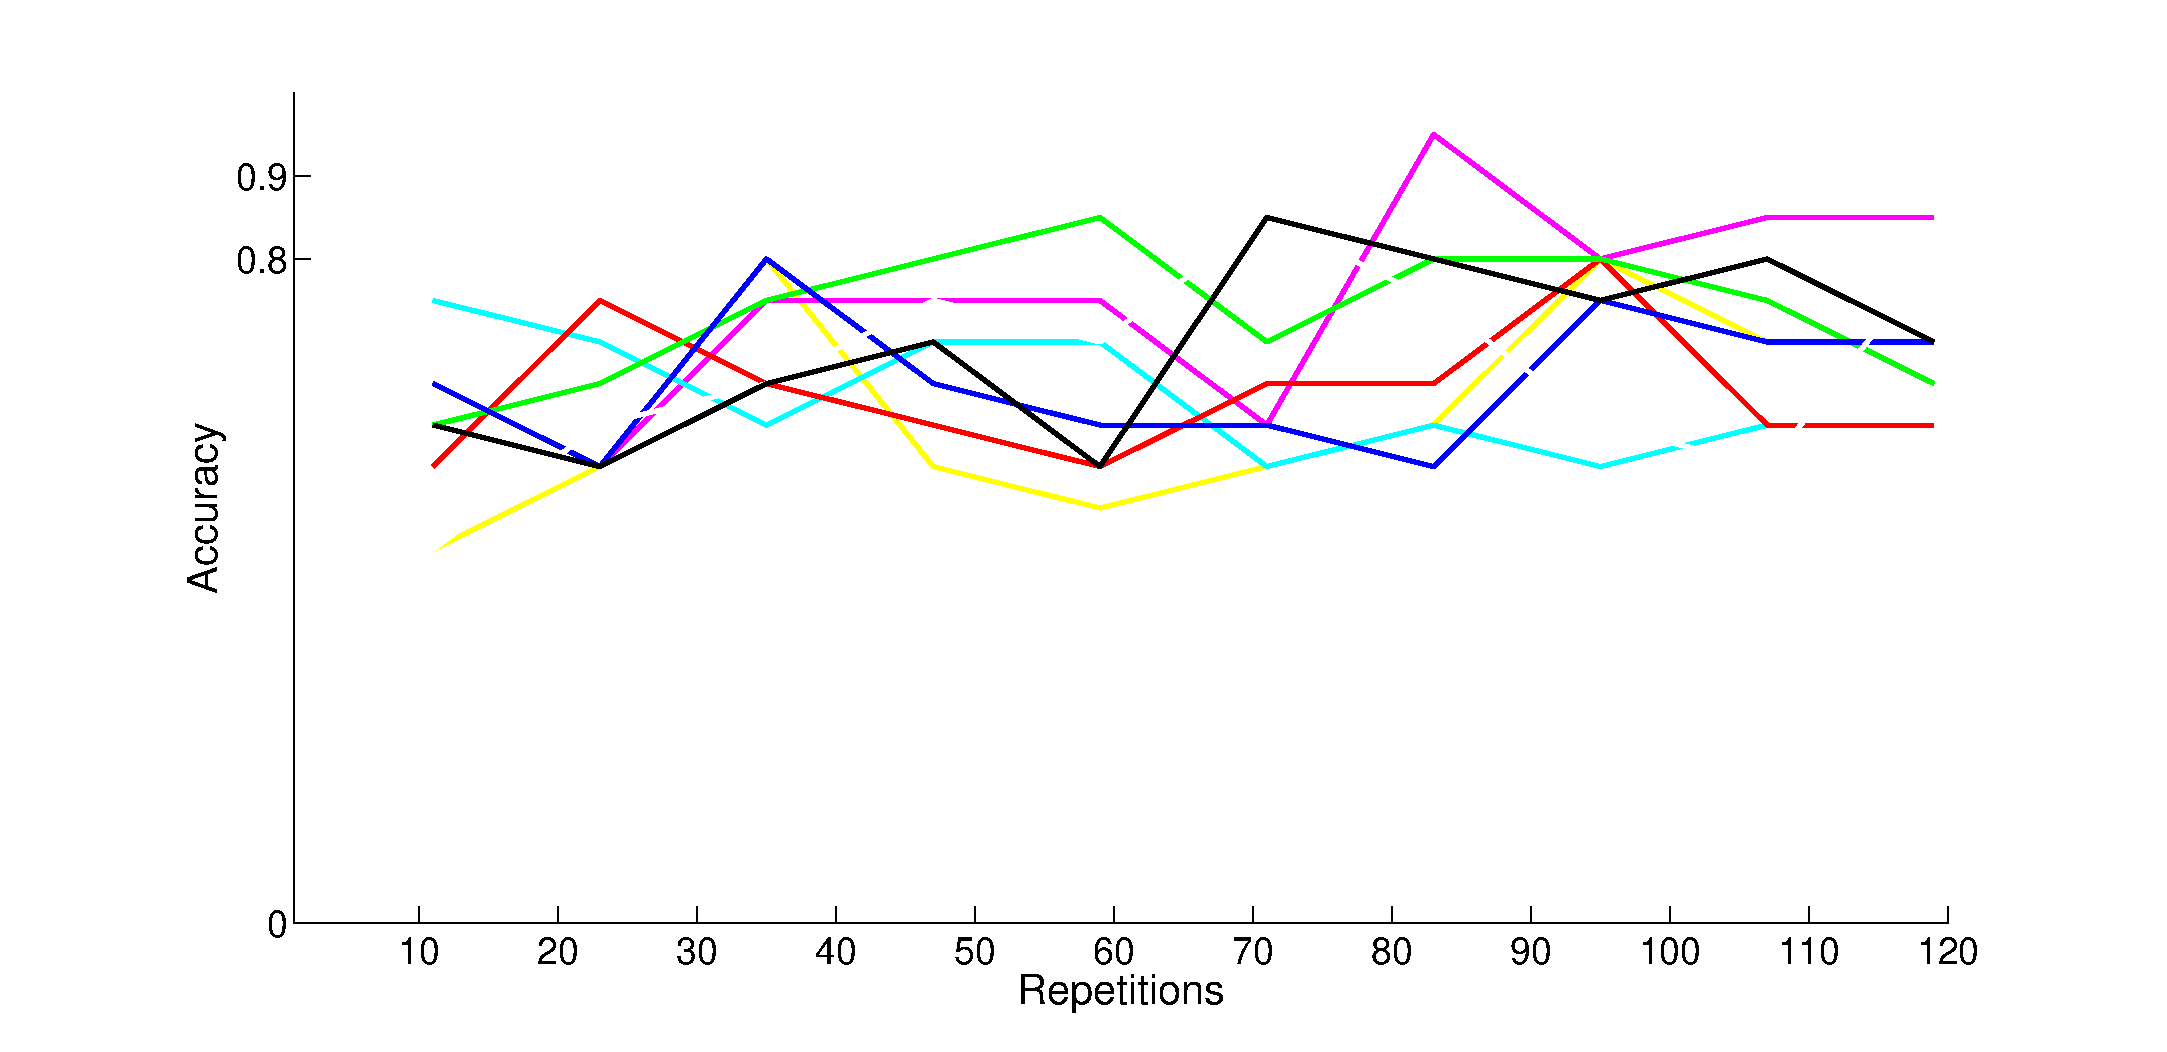
\includegraphics[width=18cm]{singletriality.eps}
\caption{This is a figure, Schemes follow the same formatting. If there are multiple panels, they should be listed as: (\textbf{a}) Description of what is contained in the first panel. (\textbf{b}) Description of what is contained in the second panel. Figures should be placed in the main text near to the first time they are cited. A caption on a single line should be centered.}
\label{fig:singletrial}
\end{figure}

%%%%%%%%%%%%%%%%%%%%%%%%%%%%%%%%%%%%%%%%%%
\section{Discussion}

This method, different from other methods which is based on the nonlinearity of the gradient of histograms which can be used to detect 

is also based on how the image look like.

SNR of p300 and how to detect it

Check if you can use this to detect any kind of transient signal.

Compare if it is possible with the descriptors from one subject, discriminate the others.

Channal identification based on the metric distance between the bags


%%%%%%%%%%%%%%%%%%%%%%%%%%%%%%%%%%%%%%%%%%
\section{Conclusion}

With this result we showed a method to process EEG signals where the main characteristic can be both, rhytmic in nature as in motor imagery, and also transient and in time space, like the P300 event related potential.

If we avoid removing artefacts achieve a higher value of classification.

Si el desempeño da parecido hay que escribirlo ya que con menos valores se permite un ITR mayor.

We also achieved single trial classification for just one subject.


%%%%%%%%%%%%%%%%%%%%%%%%%%%%%%%%%%%%%%%%%%
\subsection{Subsection}

\subsubsection{Subsubsection}

Bulleted lists look like this:
\begin{itemize}[leftmargin=*,labelsep=4mm]
\item	First bullet
\item	Second bullet
\item	Third bullet
\end{itemize}

Numbered lists can be added as follows:
\begin{enumerate}[leftmargin=*,labelsep=3mm]
\item	First item
\item	Second item
\item	Third item
\end{enumerate}

The text continues here.

\subsection{Figures, Tables and Schemes}

All figures and tables should be cited in the main text as Figure 1, Table 1, etc.

\begin{figure}[H]
\centering

\includegraphics[width=9cm]{subjectaveraged.eps}
\caption{This is a figure, Schemes follow the same formatting. If there are multiple panels, they should be listed as: (\textbf{a}) Description of what is contained in the first panel. (\textbf{b}) Description of what is contained in the second panel. Figures should be placed in the main text near to the first time they are cited. A caption on a single line should be centered.}
\end{figure}   


\subsection{Formatting of Mathematical Components}

This is an example of an equation:

\begin{equation}
\mathbb{S}
\end{equation}

%% If the documentclass option "submit" is chosen, please insert a blank line before and after any math environment (equation and eqnarray environments). This ensures correct linenumbering. The blank line should be removed when the documentclass option is changed to "accept" because the text following an equation should not be a new paragraph. 
Please punctuate equations as regular text. Theorem-type environments (including propositions, lemmas, corollaries etc.) can be formatted as follows:
%% Example of a theorem:
\begin{Theorem}
Example text of a theorem.
\end{Theorem}

The text continues here. Proofs must be formatted as follows:

%% Example of a proof:
\begin{proof}[Proof of Theorem 1]
Text of the proof. Note that the phrase `of Theorem 1' is optional if it is clear which theorem is being referred to.
\end{proof}
The text continues here.

%%%%%%%%%%%%%%%%%%%%%%%%%%%%%%%%%%%%%%%%%%
\section{Discussion}

Authors should discuss the results and how they can be interpreted in perspective of previous studies and of the working hypotheses. The findings and their implications should be discussed in the broadest context possible. Future research directions may also be highlighted.

%%%%%%%%%%%%%%%%%%%%%%%%%%%%%%%%%%%%%%%%%%
\section{Materials and Methods}

Materials and Methods should be described with sufficient details to allow others to replicate and build on published results. Please note that publication of your manuscript implicates that you must make all materials, data, computer code, and protocols associated with the publication available to readers. Please disclose at the submission stage any restrictions on the availability of materials or information. New methods and protocols should be described in detail while well-established methods can be briefly described and appropriately cited.

Research manuscripts reporting large datasets that are deposited in a publicly available database should specify where the data have been deposited and provide the relevant accession numbers. If the accession numbers have not yet been obtained at the time of submission, please state that they will be provided during review. They must be provided prior to publication.

Interventionary studies involving animals or humans, and other studies require ethical approval must list the authority that provided approval and the corresponding ethical approval code. 

%%%%%%%%%%%%%%%%%%%%%%%%%%%%%%%%%%%%%%%%%%
\section{Conclusions}

This section is not mandatory, but can be added to the manuscript if the discussion is unusually long or complex.

%%%%%%%%%%%%%%%%%%%%%%%%%%%%%%%%%%%%%%%%%%
\vspace{6pt} 

%%%%%%%%%%%%%%%%%%%%%%%%%%%%%%%%%%%%%%%%%%
%% optional
\supplementary{The following are available online at www.mdpi.com/link, Figure S1: title, Table S1: title, Video S1: title.}

%%%%%%%%%%%%%%%%%%%%%%%%%%%%%%%%%%%%%%%%%%
\acknowledgments{This project was supported by the ITBACyT-15 funding program issued by ITBA University.}

%%%%%%%%%%%%%%%%%%%%%%%%%%%%%%%%%%%%%%%%%%
\authorcontributions{Juan Miguel Santos organized the project and conceived the idea. All the authors equally worked in the completion of this project.}

%%%%%%%%%%%%%%%%%%%%%%%%%%%%%%%%%%%%%%%%%%
\conflictofinterests{The authors declare no conflict of interest.} 

%%%%%%%%%%%%%%%%%%%%%%%%%%%%%%%%%%%%%%%%%%
%% optional
\abbreviations{The following abbreviations are used in this manuscript:\\

\noindent MDPI: Multidisciplinary Digital Publishing Institute\\
DOAJ: Directory of open access journals\\
TLA: Three letter acronym\\
LD: linear dichroism}

%%%%%%%%%%%%%%%%%%%%%%%%%%%%%%%%%%%%%%%%%%
%% optional
\appendixtitles{no} %Leave argument "no" if all appendix headings stay EMPTY (then no dot is printed after "Appendix A"). If the appendix sections contain a heading then change the argument to "yes".
\appendixsections{multiple} %Leave argument "multiple" if there are multiple sections. Then a counter is printed ("Appendix A?). If there is only one appendix section then change the argument to ?one? and no counter is printed (?Appendix?).
\appendix
\section{}
The appendix is an optional section that can contain details and data supplemental to the main text. For example, explanations of experimental details that would disrupt the flow of the main text, but nonetheless remain crucial to understanding and reproducing the research shown; figures of replicates for experiments of which representative data is shown in the main text can be added here if brief, or as Supplementary data. Mathemtaical proofs of results not central to the paper can be added as an appendix.

\section{}
All appendix sections must be cited in the main text. In the appendixes, Figures, Tables, etc. should be labeled starting with `A', e.g., Figure A1, Figure A2, etc. 

%%%%%%%%%%%%%%%%%%%%%%%%%%%%%%%%%%%%%%%%%%
% Citations and References in Supplementary files are permitted provided that they also appear in the reference list here. 
\bibliographystyle{mdpi}

%=====================================
% References, variant A: internal bibliography
%=====================================
%\renewcommand\bibname{References}
%\begin{thebibliography}{999}
% Reference 1
%\bibitem{ref-journal}
%Lastname, F.; Author, T. The title of the cited article. {\em Journal Abbreviation} {\bf 2008}, {\em 10}, 142-149.
% Reference 2
%\bibitem{ref-book}
%Lastname, F.F.; Author, T. The title of the cited contribution. In {\em The Book Title}; Editor, F., Meditor, A., Eds.; Publishing House: City, Country, 2007; pp. 32-58.
%\end{thebibliography}

%=====================================
% References, variant B: external bibliography
%=====================================
\bibliography{article}

%%%%%%%%%%%%%%%%%%%%%%%%%%%%%%%%%%%%%%%%%%
%% optional
\sampleavailability{Samples of the compounds ...... are available from the authors.}

%%%%%%%%%%%%%%%%%%%%%%%%%%%%%%%%%%%%%%%%%%
\end{document}

